\section{Model-Based Safety Analysis}

\mike{Audience should already know about model-based safety analysis.  We want to discuss two ``strands'' of MBSA, one with explicit fault propagation of faults rather than system dynamics, and another based on faults propagating through their effects on dynamics}.

A model-based approach for safety analysis was first proposed by Joshi et. al in \cite{Joshi05:Dasc, Joshi05:SafeComp, Joshi07:Hase}.  In this approach, a safety analysis system model (SASM) is the central artifact in the safety analysis process, and traditional safety analysis artifacts, such as fault trees, are automatically generated by tools that analyze the SASM. Figure~\mike{include figure?} \danielle{Return to this, Danielle} provides an overview of this process applied to the wheel braking system example.

The contents and structure of the SASM differ significantly across different conceptions of MBSA.  We can draw broad outlines between two different approaches: one in which {\em faults} are propagated between components explicitly and the analysis proceeds by determining the likelihood of faults to system boundaries, and another in which faults propagate by changing the system dynamics, which may cause the system behavior to visibly change.  We call the first style the {\em explicit fault propagation} and the second style {\em implicit fault propagation} or {\em behavioral} propagation.

We contrast these two styles below...

\mike{Regurgitate content from "Model-Based Safety Analysis with smartIflow"}
\danielle{I added the citation from this paper to the bib file: cite\{info17:HaLuHo\} in case we want to use it.} \cite{info17:HaLuHo}.

\mike{Some contrasting points: richness of dynamics.  Most tools use formalisms that can only represent discrete quantities; we can do real-valued or large-domain integer dynamics}


\mike{Also we are explicitly integrated with an architecture language}


\subsection{Explicit Fault Propagation Approaches}



\mike{What is being done in AltaRica, HiPHOPS, AADL Error Annex...more here about primacy of faults as the mechanism of propagation between components.  Steal from proposal.}
\danielle{I added a few things from the proposal regarding fault propagation between components. There is a note below where that begins. I am not sure which papers you are referring to here so I can't really dig into those...}

The explicit propagation approach focuses on faults rather than constructing a model of system dynamics.

We illustrate this approach with the AADL error model annex~\cite{SAEAS} that can be used to describe system behaviors in the presence of faults. This annex has facilities for defining error types which can be used to describe error events that indicate errors in the system. The behavior of system components in the presence of errors is determined by state machines that are attached to system components; these state machines can determine error propagations and error composition for systems created from various subcomponents.

Error types in this framework are a set of enumeration values such as NoData, BadData, LateDelivery, EarlyDelivery, TimingError, and NoService. These errors can be arranged in a hierarchy. For example, LateDelivery and EarlyDelivery are subtypes of TimingError. The errors do not have any information (other than their type) associated with them. AADL includes information on the bindings of logical components (processes, threads, systems) and their communication mechanisms onto physical resources (memories, processors, busses), and the error annex uses this information to describe how physical failures can manifest in logical components.

\begin{figure}
  \centering
 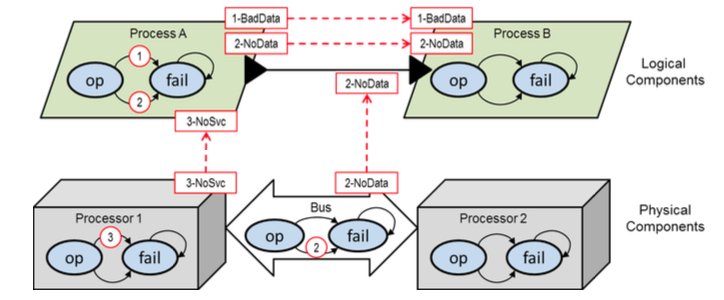
\includegraphics[width=0.75\textwidth]{images/error_annex.png}
  \vspace{-0.1in}
  \caption{Example of Error Model Information and Propagation}
  \label{fig:error_annex}
\end{figure}

An example is shown in Figure~\ref{fig:error_annex} \mike{Where is this figure?!?} \danielle{It was in the MBSA section. I have moved it here and if needed will reference from there}. Errors are described by the red rectangles labeled with error types: 1-BadData, 2-NoData, 3-NoSvc. Error events that can cause a component to fail are labeled with the corresponding error number. The error behavior of components is described by their state machines. Note that while all state machines in Figure 2 have two states, they can be much more complex. The red dashed arrows indicate propagations describing how failures in one component can cause other components to fail. For example, failures in the physical layer propagate to failures in the associated logical components.

Although the error model annex is very capable, it is not closely tied to the behavioral model of components or their requirements. For example, in the wheel braking system (WBS) example \cite{AIR6110}, it is possible that hydraulic system valves can fail open or fail closed. In fail closed, downstream components receive no flow and upstream pipes may become highly pressurized as a natural consequence of the failure. Physical models of these behavioral relationships often exist that can propagate failures in terms of the behavioral relationships between components. However, with the AADL error model annex, the propagations must be (re)specified and defined for each component. The user must therefore model the system twice, specifying propagations in the models of the physical phenomena, and again using enumerations and propagation rules in state machines in the error model annex. This re-specification can lead to inconsistencies between physical models and error annex models. In addition, the physical relationships between failures can be complex and may not be describable using enumeration values, leading to additional inconsistencies between the behavior of the physical phenomenon and the behavior of the error model.

\danielle{Added from proposal. I believe this describes what you mentioned above, Mike.}
This research attempts to bridge the descriptions of errors in the error model annex with behavioral descriptions of components. We start from the error model notions of error types and state machines that describe transitions from nominal to error states. However, we then tie these nominal and error states to behavioral models of the components in question that describe how the faults manifest themselves in terms of the signals or quantities produced by the components. Now the behavioral models can provide implicit propagation of the faulty behaviors and the natural consequences of failures on component behavior will be manifested in the propagation of other component faults through the behavioral model.

To accomplish this, we use AADL and the error model annex to describe faults and to use the AGREE contract specification language to describe behavioral models. This will require extensions to AGREE to define fault models that describe how different faults manifest themselves in changes to output signals. It will also require changes to the error annex. The conditions under which faults occur will become richer such that they describe not just propagation of enumerations from other components, but also valuations of input signals. For example, very high pressure in a pipe in the WBS model may lead to a \textit{pipe burst} failure. 


\subsection{Implicit Fault Propagation Approaches (Behavioral MBSA)}

\mike{Unfortunately, this is what is done, and done well in xSAP; they have a CAV paper on it; need to account for this}.
\danielle{I have been trying to find this paper... not sure what it is. I will move on for now and perhaps you have the paper title so that I can add a citation and some accounting for their research.}

The analysis starts from a {\em nominal} model of the system that describes the system behavior when no faults are present.  To perform safety analysis, we then also formalize the fault model. The fault model, in addition to common failure modes like \emph{non-deterministic}, \emph{inverted}, \emph{stuck\_at} etc, could encode information
regarding fault propagation, simultaneous dependent faults and fault hierarchies, etc.
After specifying the fault model and composing it with the original system model, the safety analysis involves verifying whether the safety requirements hold in presence of the faults defined in the fault model.


In this work, a behavior fault modeling language was constructed as an extension to the Lustre language \cite{Halbwachs91:IEEE}. Lustre is the kernel language of the popular model-based development tool SCADE \cite{SCADE}. In this approach, a safety engineer can model different kinds of fault behavior: e.g., stuck-at, ramp-up, ramp-down, and nondeterministic, and then {\em weave} these fault models into the nominal model. The language for describing faults is extensible, allowing engineers to define a catalog of faults appropriate for their domain. In addition, the weaving process allows error propagation between unconnected components within a system model \cite{Joshi07:Hase}. This allows consideration of physical aspects (e.g., proximity of components, shared resources such as power) that may not be present in a logical system model but can lead to dependent failures. In addition, it allows propagation of faults in the reverse direction of the model data flow. This can occur when physical components have coupling such as back-pressure in fluid systems or power surges in the opposite direction of communication through connected components. Finally, it is possible to create fault mediations to describe the output in the presence of multiple simultaneous faults.



%In previous work, component-level modeling tools such as Simulink \cite{MathWorks} and SCADE \cite{SCADE} were extended. In this work, we adapt this process to target system architecture models \cite{AADL, SysML} for safety analysis.

%\subsection{Safety Analysis Approach}
\begin{figure}
  \centering
 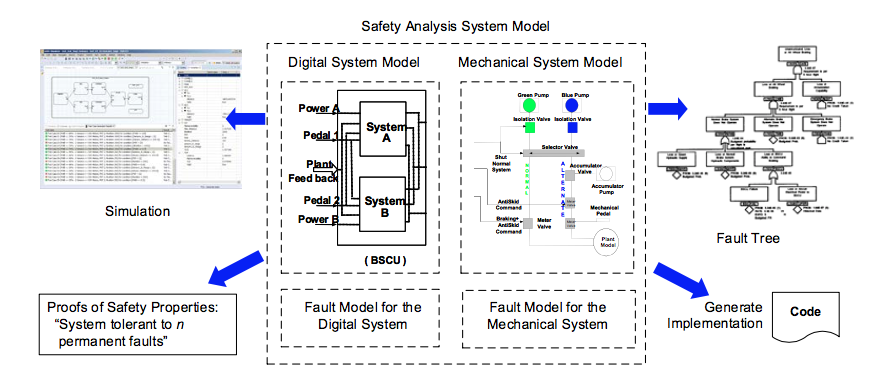
\includegraphics[width=1\textwidth]{images/SASM.png}
  \vspace{-0.1in}
  \caption{Safety Analysis System Model}
  \label{fig:sasm}
\end{figure}

A safety analysis system model can be used for a variety of simulations and analyses as shown in Figure~\ref{fig:sasm} \mike{include figure?} \danielle{Do you mean a figure like this one? If not, I can change it (I got it from the proposal) If so, perhaps Darren has a nonblurry copy of the figure? I can't get this one to be more clear...}. Modeling allows trivial exploration of \textit{what-if} scenarios involving combinations of faults through simulations. For more rigorous analyses, static analysis tools, such as model checkers and theorem provers, can be used to automatically prove (or disprove) whether the system meets specific safety requirements.
The primary approach used for analysis in previous work was model checking. After creating the system model, a model checker was used to verify that safety properties hold on the nominal system, an idealized model of the digital controller and the mechanical system containing no faults. Once the nominal model is shown to satisfy the safety property, the behavior of the fault-extended model can be examined. In the approach described by Joshi et al. in \cite{Joshi05:Dasc, Joshi05:SafeComp, Joshi07:Hase}, this analysis was performed by determining whether the property held for a given fault threshold: the maximum number of component faults to which the system is expected to be resilient.

This fault threshold is, in some sense, an approximation of the likelihood of component faults. It maps from the probabilistic \textit{real world} potential for component failure into a non-probabilistic verification problem. Recent work \cite{CAV2015:BoCiGrMa} uses a more sophisticated approach involving minimum cut sets to describe the set of potential component failures that must be considered. Both approaches provide separation between the probabilistic aspects of the real world and the computational demands of formal analysis. This approach currently scales far better than direct use of probabilistic model checking tools such as PRISM \cite{CAV2011:KwNoPa}, and will likely continue to do so in the future.

\iffalse
\subsection{Compositional Verification of System Architectures}

As part of the NASA Compositional Verification of Flight Critical Systems (CVFCS) project and the DARPA META and High Assurance Cyber Military Systems (HACMS) projects, we have constructed sophisticated compositional verification tools for reasoning about complex systems architectures. These tools \cite{NFM2012:CoGaMiWhLaLu} allow scaling of formal verification through splitting the analysis of a complex system architecture into a collection of verification tasks that correspond to the structure of the architecture. By decomposing the verification effort into proofs about each subsystem within the architecture, the analysis has been scaled to very large system designs \cite{QFCS15:backes}. In the case of the software for a complex medical drug infusion pump, a monolithic analysis of the design does not terminate in 24 hours, while the compositional approach completes in just over five minutes.
<<<<<<< HEAD
The approach naturally supports an architecture-based notion of requirements refinement based on assume-guarantee contracts. The properties of components necessary to prove a system-level property, including any assumptions about the component environment, in effect define the requirements for those components. The approach allows reuse of the verification that must already be performed on safety-critical software components and enables distributed development by establishing the formal contracts for components that are used to assemble a system architecture. If we are able to establish a system property using only the contracts of its components, we have the means for performing virtual integration of the components. We can use the contract of each component as a specification for suppliers and have a great deal of confidence that if all the suppliers meet their specifications, the integrated system will work properly.
We have implemented this assume-guarantee mechanism for compositional verification as an extension of the AADL language derived from the safety property subset of the property specification language (PSL) \cite{IEEE:PSL}. The Assume-Guarantee Reasoning Environment (AGREE) is our tool for compositional verification of these contracts. Under the CVFCS project, we are currently adding automated bi-directional translation between AGREE contracts and implementation-level properties in languages such as C and Simulink. Initially, we will support translation into MATLAB properties for analysis using the Simulink Design Verifier and C assertions for analysis using source code model checkers (such as CMBC) or test- based verification. Since contracts are abstractions of component implementations, they provide a much more efficient way of representing heterogeneous components in the system model than translating the component models themselves.
=======

The approach naturally supports an architecture-based notion of requirements refinement based on assume-guarantee contracts. The properties of components necessary to prove a system-level property, including any assumptions about the component environment, in effect define the requirements for those components. The approach allows reuse of the verification that must already be performed on safety-critical software components and enables distributed development by establishing the formal contracts for components that are used to assemble a system architecture. If we are able to establish a system property using only the contracts of its components, we have the means for performing virtual integration of the components. We can use the contract of each component as a specification for suppliers and have a great deal of confidence that if all the suppliers meet their specifications, the integrated system will work properly.

We have implemented this assume-guarantee mechanism for compositional verification as an extension of the AADL language derived from the safety property subset of the property specification language (PSL) \cite{IEEE:PSL}. The Assume-Guarantee Reasoning Environment (AGREE) is our tool for compositional verification of these contracts. Under the CVFCS project, we are currently adding automated bi-directional translation between AGREE contracts and implementation-level properties in languages such as C and Simulink. Initially, we will support translation into MATLAB properties for analysis using the Simulink Design Verifier and C assertions for analysis using source code model checkers (such as CMBC) or test- based verification. Since contracts are abstractions of component implementations, they provide a much more efficient way of representing heterogeneous components in the system model than translating the component models themselves.

>>>>>>> 705062d4005b55c503d3e85e228be8e236a1ac1e

\fi

